% 精确几何图（示例 k=3/5, A=(4,12/5), B=(2,-6/5), l:y=9x/5-24/5）。
% 点 A、B 严格位于相应渐近线上，直线 l 确为通过 A 与 B 的直线。
\begin{tikzpicture}[scale=0.72,>=stealth]
\coordinate (O) at (0,0);
\coordinate (A) at (4,2.4);
\coordinate (B) at (2,-1.2);
\fill[teal!15] (O)--(A)--(B)--cycle;
\draw[->,gray!70] (-5.3,0)--(5.6,0) node[right] {$x$};
\draw[->,gray!70] (0,-3.4)--(0,3.7) node[above] {$y$};
\draw[thick,blue!65!black] (-5.1,-3.06)--(5.4,3.24);
\draw[thick,blue!65!black] (-5.1,3.06)--(5.4,-3.24);
\draw[orange!85!black,line width=1.25pt] (1,-3)--(4.5,3.3);
\draw[teal!80!black,line width=0.8pt] (O)--(A)--(B)--cycle;
\fill (O) circle(2.4pt) node[below left] {$O$};
\fill[red!85!black] (A) circle(2.7pt) node[above left=3pt] {$A(x_1,kx_1)$};
\fill[red!85!black] (B) circle(2.7pt) node[below right=3pt] {$B(x_2,-kx_2)$};
\node[blue!65!black,above right] at (4.15,2.49) {$y=kx$};
\node[blue!65!black,below right] at (3.85,-2.4) {$y=-kx$};
\node[orange!85!black,left] at (2.58,-2.19) {$\ell$};
\node[fill=white,fill opacity=.95,text opacity=1,rounded corners=1pt]
 at (-3.1,-2.45) {$k=\dfrac ba>0$};
\end{tikzpicture}
